\documentclass[12pt,a4paper]{article}
\usepackage[utf8]{inputenc}
\usepackage[indonesian]{babel}
\usepackage{graphicx}
\usepackage{hyperref}
\usepackage{geometry}
\usepackage{listings}
\usepackage{xcolor}
\usepackage{float}

\geometry{
    a4paper,
    left=3cm,
    right=3cm,
    top=3cm,
    bottom=3cm,
}

\hypersetup{
    colorlinks=true,
    linkcolor=blue,
    filecolor=magenta,      
    urlcolor=cyan,
    pdftitle={Laporan Kuis 3 PBO},
}

\title{\textbf{Laporan Kuis 3 Pemrograman Berorientasi Objek}}
\author{
    \textbf{Fransiscus Asisi Kananda Herdion Dharmawan} \\
    NIM: 24.83.1107 \\
    Teknik Komputer \\
    Universitas Amikom Yogyakarta
}
\date{\today}

\begin{document}

\maketitle

\section*{Informasi Proyek}
Kode sumber lengkap dan *repository* dari tugas ini dapat diakses pada tautan GitHub berikut: \\
\url{https://github.com/diondharmawan/Amikom-Tugas-Kuis_3_PBO}

\section{Jawaban Soal 1: Abstraksi}
\textbf{Pertanyaan:} Jelaskan bagaimana Anda menerapkan Abstraksi menggunakan \textit{Abstract Base Class} (ABC) di Python untuk membuat kelas induk bernama \texttt{RekeningBank}. Tuliskan kerangka kelasnya saja, serta tentukan \textit{abstract method} apa yang harus ada.

\textbf{Jawaban:} \\
Abstraksi diterapkan dengan membuat kelas \texttt{RekeningBank} yang mewarisi \texttt{ABC} (\textit{Abstract Base Class}) dari modul bawaan Python \texttt{abc}. Hal ini mencegah kita untuk membuat instansiasi langsung dari kelas \texttt{RekeningBank}. Karena regulasi mewajibkan prosedur standar perhitungan biaya administrasi bulanan dan pencetakan laporan ringkas, maka \textit{abstract method} yang harus ada adalah \texttt{hitung\_biaya\_admin()} dan \texttt{cetak\_laporan()}. Metode ini memaksa setiap subclass (seperti Giro dan Tabungan) untuk mengimplementasikan logikanya masing-masing.

\begin{figure}[H]
    \centering
    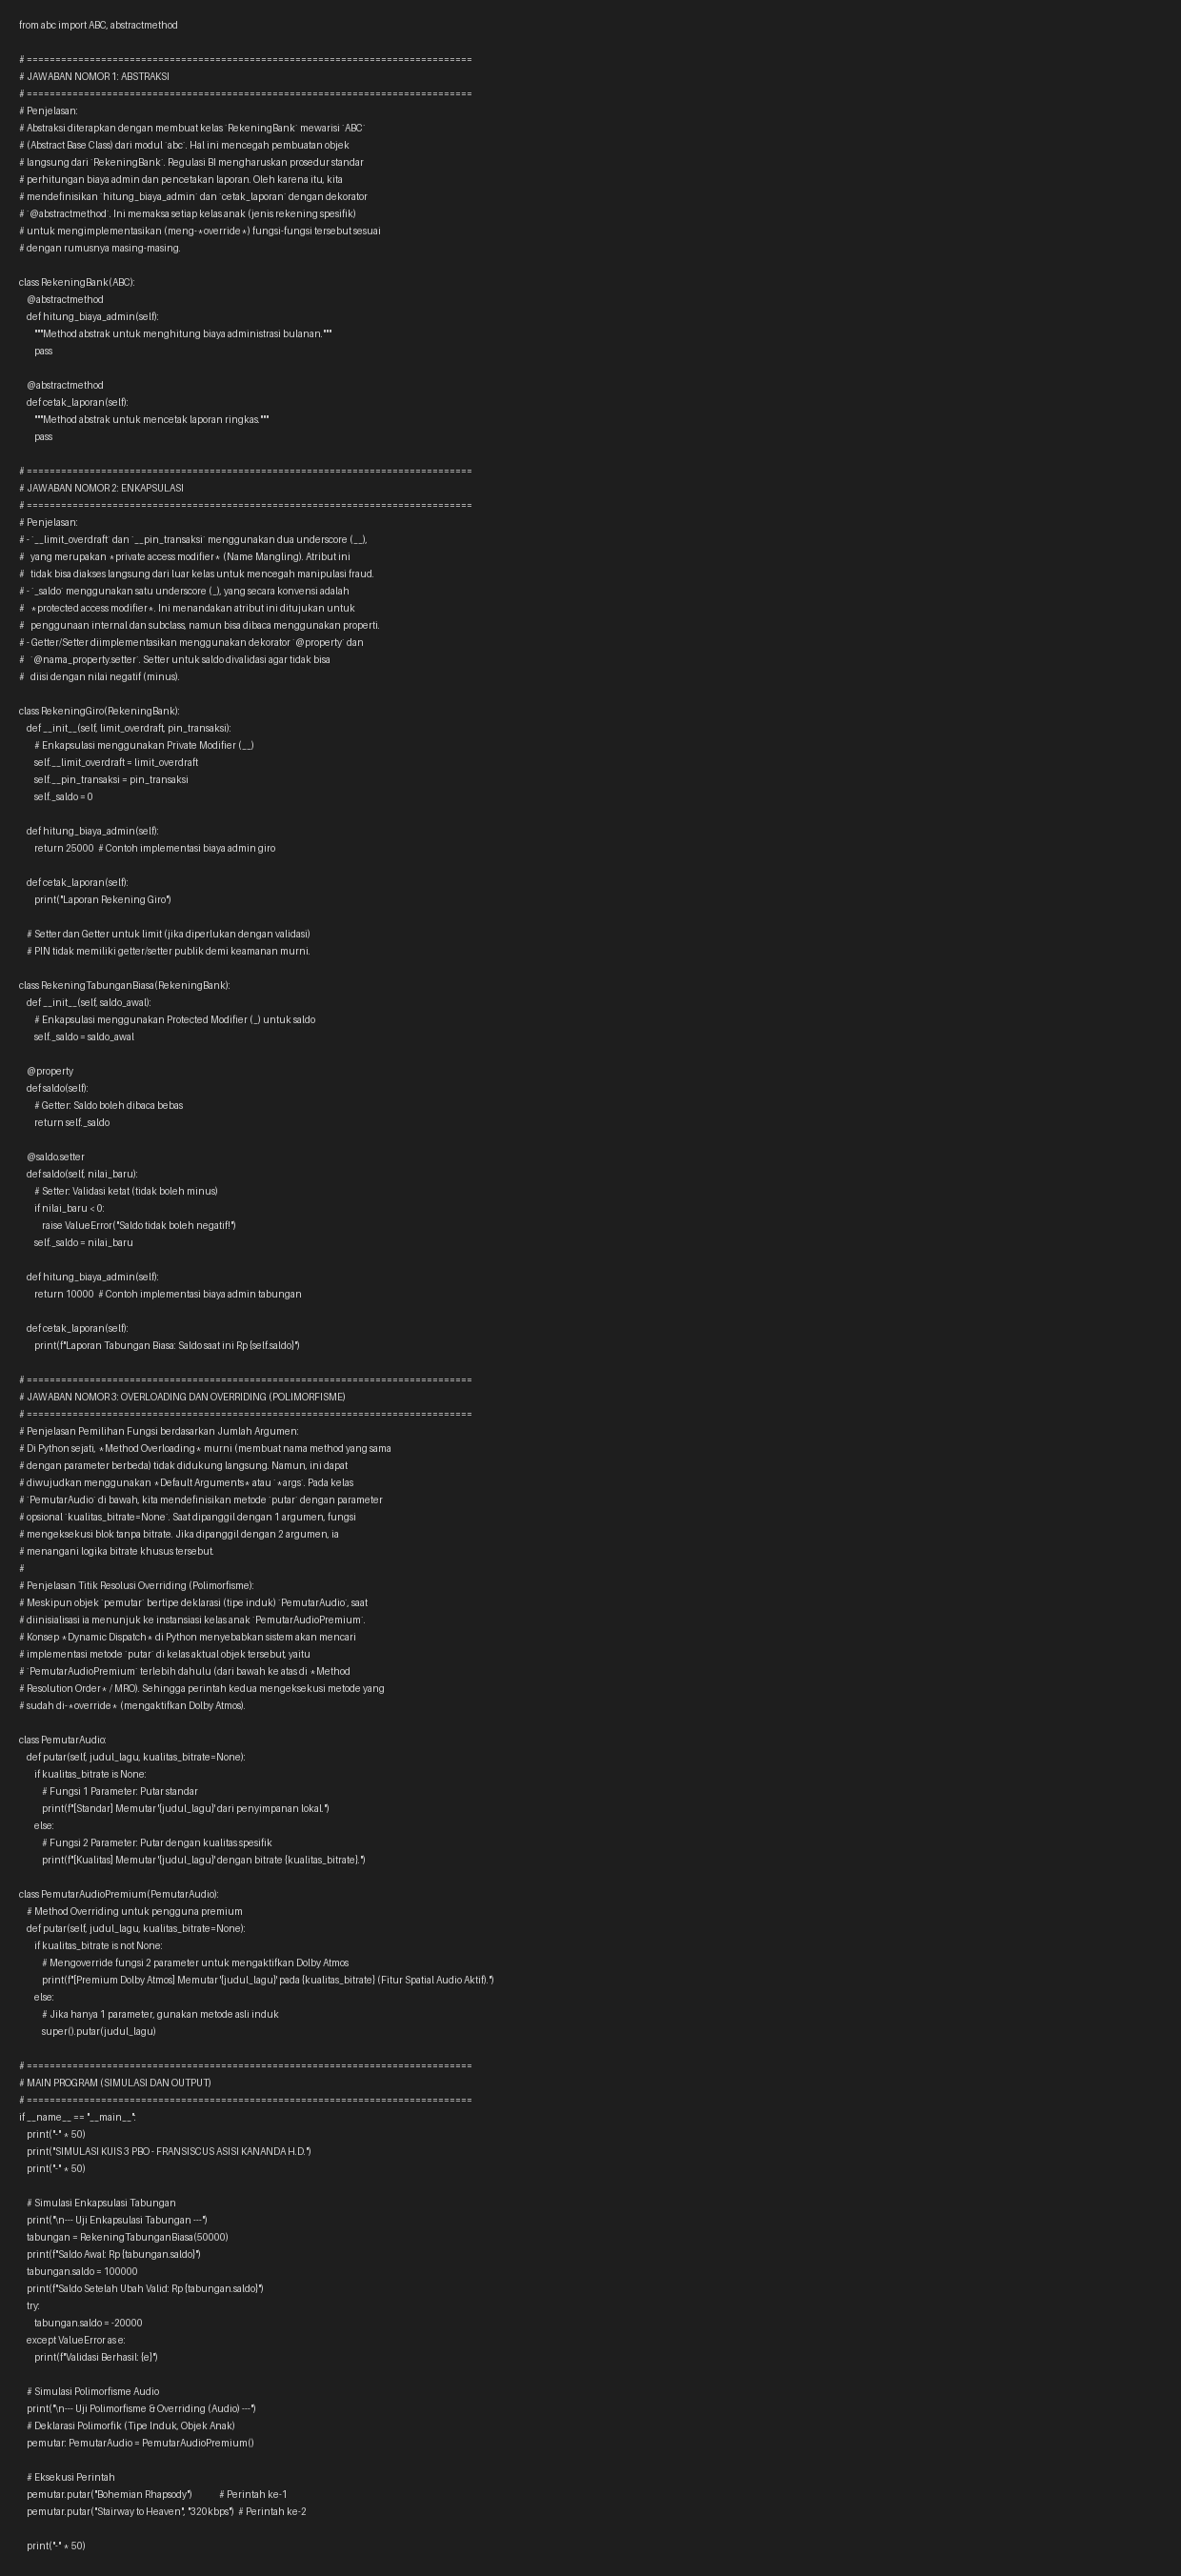
\includegraphics[width=0.8\textwidth]{sc_code.png}
    \caption{Tangkapan layar kerangka kelas (Source Code)}
\end{figure}

\section{Jawaban Soal 2: Enkapsulasi}
\textbf{Pertanyaan:} Jelaskan strategi Enkapsulasi pada \texttt{RekeningGiro} dan \texttt{RekeningTabunganBiasa}. Gambarkan/tuliskan pemanfaatan Access Modifier (\texttt{\_} vs \texttt{\_\_}) dan Getter/Setter.

\textbf{Jawaban:} \\
Pada kelas \texttt{RekeningGiro}, data sensitif berupa limit overdraft dan PIN diamankan menggunakan \textit{Private Access Modifier} (\texttt{\_\_limit\_overdraft} dan \texttt{\_\_pin\_transaksi}). Python melakukan \textit{name mangling} untuk ini sehingga atribut tersebut sulit diakses langsung dari luar objek untuk mencegah \textit{fraud}.

Pada \texttt{RekeningTabunganBiasa}, atribut \texttt{\_saldo} dilindungi dengan \textit{Protected Access Modifier} (menggunakan satu underscore). Akses baca diperbolehkan secara bebas menggunakan properti Getter (\texttt{@property def saldo}). Namun untuk mengubah (menulis), nilai harus dilewatkan melalui fungsi Setter (\texttt{@saldo.setter def saldo}) yang di dalamnya terdapat logika validasi ketat untuk memastikan saldo tidak dimasukkan dengan nilai negatif (minus).

\section{Jawaban Soal 3: Overloading dan Polimorfisme}
\textbf{Pertanyaan:} Tunjukkan bagaimana sistem memilih fungsi berdasarkan jumlah argumen, dan tunjukkan bagaimana sistem menentukan bahwa perintah kedua mengarah ke kelas anak meskipun dideklarasikan sebagai induk.

\textbf{Jawaban:} \\
Di Python, \textit{Method Overloading} murni seperti di Java (di mana nama fungsi sama namun argumennya berbeda-beda deklarasinya secara eksplisit) tidak didukung langsung. Namun hal ini dapat dicapai melalui parameter default (\textit{default arguments}) atau \texttt{*args}. Metode \texttt{putar(self, judul\_lagu, kualitas\_bitrate=None)} akan mendeteksi apabila argumen kedua dikirimkan. Jika dipanggil dengan 1 argumen, parameter kedua bernilai \texttt{None}, memicu pemutaran lokal. Jika 2 argumen dipanggil, ia mengenali spesifikasi bitrate.

Titik resolusi \textit{Overriding} (Polimorfisme) terjadi secara dinamis. Saat objek dideklarasikan secara polimorfik (tipe variabel dianggap \texttt{PemutarAudio} tetapi diset sebagai instance \texttt{PemutarAudioPremium}), Python menggunakan \textit{Dynamic Dispatch}. Eksekusi pemanggilan metode akan mencari pada \textit{Method Resolution Order} (MRO) dari bawah (dari kelas aktualnya terlebih dahulu) ke atas. Sehingga saat dipanggil, fungsi \texttt{putar} pada kelas anak \texttt{PemutarAudioPremium} lah yang terpicu, dan fitur \textit{Dolby Atmos} otomatis aktif.

\begin{figure}[H]
    \centering
    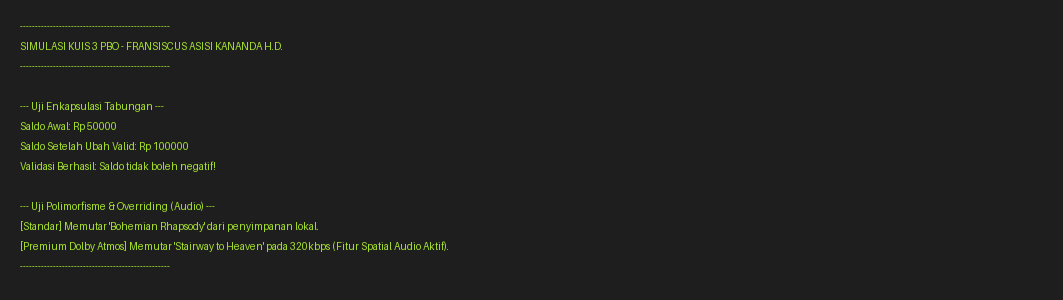
\includegraphics[width=0.8\textwidth]{sc_output.png}
    \caption{Tangkapan layar hasil simulasi / output eksekusi}
\end{figure}

\section{Kesimpulan}
Tugas Kuis 3 PBO ini mendemonstrasikan implementasi empat pilar utama Pemrograman Berorientasi Objek di Python, yaitu Abstraksi, Enkapsulasi, Pewarisan, dan Polimorfisme (Overloading \& Overriding). Penulisan kode Python disesuaikan untuk mengatasi limitasi bahasa (seperti pada Method Overloading) dengan menggunakan teknik *best-practice* Pythonik (seperti \textit{default parameters} dan \textit{Dynamic Dispatch}).

\end{document}
